
\documentclass{exam}

\usepackage{units} 
\usepackage{graphicx}
\usepackage[fleqn]{amsmath}
\usepackage{cancel}
\usepackage{float}
\usepackage{mdwlist}
\usepackage{booktabs}
\usepackage{cancel}
\usepackage{polynom}
\usepackage{caption}
\usepackage{fullpage}
\usepackage{xfrac}
\usepackage{enumerate}

\newcommand{\degree}{\ensuremath{^\circ}} 
\everymath{\displaystyle}

% \begin{figure}[H]
%   \centering
%   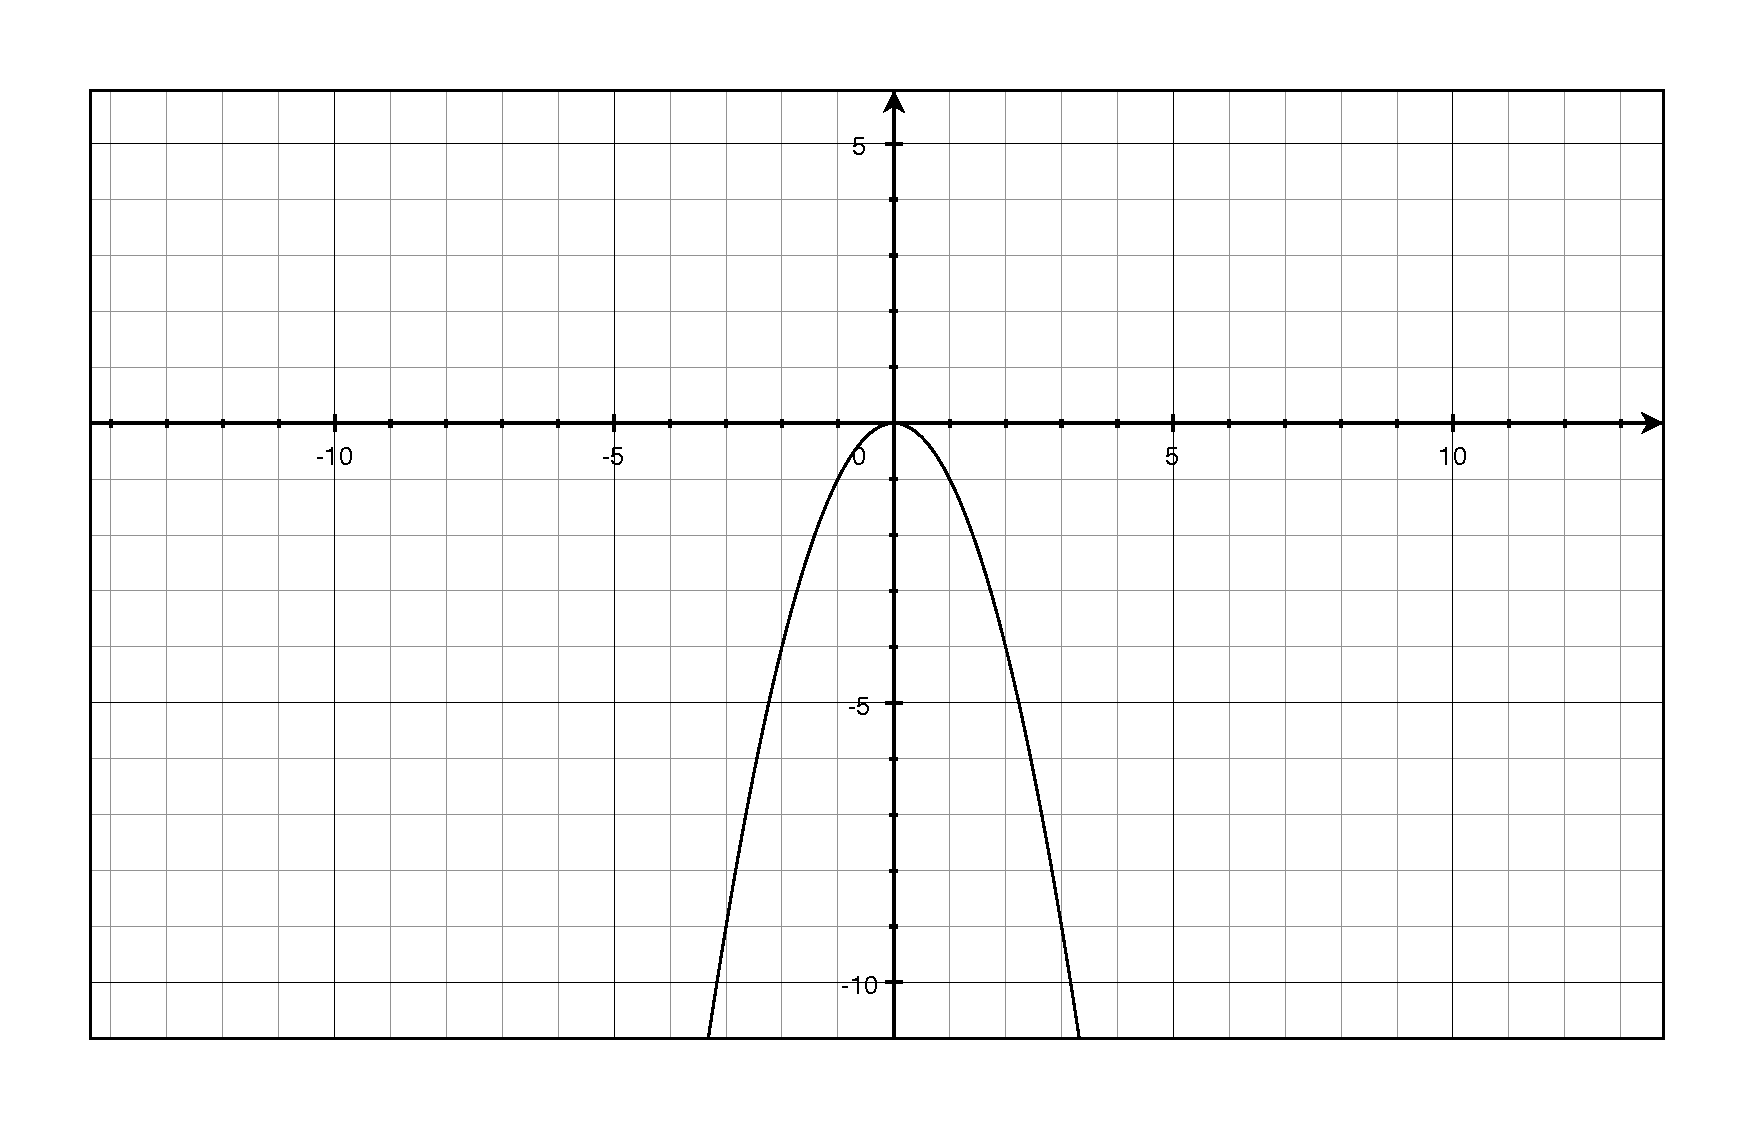
\includegraphics[scale=0.9]{problem7.eps}
%   \caption*{Problem 7}
% \end{figure}

% \begin{tabular}{cc}
%   \toprule
%   period & amplitude \\
%   \midrule
%   value one & value two
%   \bottomrule
% \end{tabular}

% \printanswers

\ifprintanswers 
  \usepackage{2in1, lscape} 
\fi

\date{June 17, 2013}
\author{}
\title{Math 141 \\ Homework 15}

\begin{document}

  \maketitle

  \section{Homework}

  Section 4.3: TO DO

 \section{Extra Credit}
  Section 4.2: TO DO

  \ifprintanswers
    \begin{description}
      \item[75]
        answer here
    \end{description}
  \fi

  \section{Review}

  \begin{enumerate}

    \item $f(x) = x^3 - 1$ 

  \end{enumerate}

  \ifprintanswers
    \section{Section 4.3}

    \begin{description}

      \item[3] 
        \begin{align*}
          5^2 &= 25 \\
          5^0 &= 1 \\
        \end{align*}

    \end{description}

  \else
    \vspace{2 cm}
    \begin{quote}
      \begin{em}
        TO DO
      \end{em}
    \end{quote}

    \hspace{1 cm} --Carl Jung
  \fi

\end{document}

